\documentclass[letta4 paper]{article}
% Set target color model to RGB
\usepackage[inner=2.0cm,outer=2.0cm,top=2.5cm,bottom=2.5cm]{geometry}
\usepackage{setspace}
\usepackage[rgb]{xcolor}
\usepackage{verbatim}
\usepackage{subcaption}
\usepackage{amsgen,amsmath,amstext,amsbsy,amsopn,tikz,amssymb,tkz-linknodes}
\usepackage{fancyhdr}
\usepackage[colorlinks=true, urlcolor=blue,  linkcolor=blue, citecolor=blue]{hyperref}
\usepackage[colorinlistoftodos]{todonotes}
\usepackage{rotating}
\usepackage{listings}
\usepackage{algorithm}
\usepackage{algorithmic}
\lstset{
%	language=bash,
	basicstyle=\ttfamily
}

\newcommand{\ra}[1]{\renewcommand{\arraystretch}{#1}}

\newtheorem{thm}{Theorem}[section]
\newtheorem{prop}[thm]{Proposition}
\newtheorem{lem}[thm]{Lemma}
\newtheorem{cor}[thm]{Corollary}
\newtheorem{defn}[thm]{Definition}
\newtheorem{rem}[thm]{Remark}
\numberwithin{equation}{section}
\graphicspath{ {./img/} }

\newcommand{\homework}[6]{
   \pagestyle{myheadings}
   \thispagestyle{plain}
   \newpage
   \setcounter{page}{1}
   \noindent
   \begin{center}
   \framebox{
      \vbox{\vspace{2mm}
    \hbox to 6.28in { {\bf F1TENTH Autonomous Racing \hfill {\small (#2)}} }
       \vspace{6mm}
       \hbox to 6.28in { {\Large \hfill #1  \hfill} }
       \vspace{6mm}
       \hbox to 6.28in { {\it Instructor: {\rm #3} \hfill Name: {\rm #5}, StudentID: {\rm #6}} }
       %\hbox to 6.28in { {\it T\textbf{A:} #4  \hfill #6}}
      \vspace{2mm}}
   }
   \end{center}
   \markboth{#5 -- #1}{#5 -- #1}
   \vspace*{4mm}
}


\newcommand{\problem}[3]{~\\\fbox{\textbf{Problem #1: #2}}\hfill (#3 points)\newline}
\newcommand{\subproblem}[1]{~\newline\textbf{(#1)}}
\newcommand{\D}{\mathcal{D}}
\newcommand{\Hy}{\mathcal{H}}
\newcommand{\VS}{\textrm{VS}}
\newcommand{\solution}{~\newline\textbf{\textit{(Solution)}} }

\newcommand{\bbF}{\mathbb{F}}
\newcommand{\bbX}{\mathbb{X}}
\newcommand{\bI}{\mathbf{I}}
\newcommand{\bX}{\mathbf{X}}
\newcommand{\bY}{\mathbf{Y}}
\newcommand{\bepsilon}{\boldsymbol{\epsilon}}
\newcommand{\balpha}{\boldsymbol{\alpha}}
\newcommand{\bbeta}{\boldsymbol{\beta}}
\newcommand{\0}{\mathbf{0}}


\usepackage{booktabs}



\begin{document}

	\homework {Lab 8: Perception and Vision}{Due Date:}{INSTRUCTOR}{}{STUDENT NAME}{ID}
	\thispagestyle{empty}
	% -------- DO NOT REMOVE THIS LICENSE PARAGRAPH	----------------%
	\begin{table}[h]
		\begin{tabular}{l p{14cm}}
		\raisebox{-2cm}{
\includegraphics[scale=0.5, height=2.5cm]{f1_stickers_01} } & \textit{This lab and all related course material on \href{http://f1tenth.org/}{F1TENTH Autonomous Racing} has been developed by the Safe Autonomous Systems Lab at the University of Pennsylvania (Dr. Rahul Mangharam). It is licensed under a \href{https://creativecommons.org/licenses/by-nc-sa/4.0/}{Creative Commons Attribution-NonCommercial-ShareAlike 4.0 International License.} You may download, use, and modify the material, but must give attribution appropriately. Best practices can be found \href{https://wiki.creativecommons.org/wiki/best_practices_for_attribution}{here}.}
		\end{tabular}
	\end{table}
	% -------- DO NOT REMOVE THIS LICENSE PARAGRAPH	----------------%
	
	\noindent \large{\textbf{Course Policy:}} Read all the instructions below carefully before you start working on the assignment, and before you make a submission. All sources of material must be cited. The University Academic Code of Conduct will be strictly enforced.
	\\
	\\
	\textbf{THIS IS A GROUP ASSIGNMENT}. Submit one from each team.\\
	
	\section{Learning outcomes}

	The following fundamentals should be understood by the students upon completion of this lab:
		
	\begin{itemize}
        \item \textit{Camera model and parameters:} You should be able to understand how the real camera model and the pin hole camera model are related and what assumptions are made while going from the former to the latter.
		\item \textit{Transformations:} You should be able to understand 3 dimensional transformations and know the representations of transformations. 
		\item \textit{Single View Geometry:} You should be able to understand and work with single view geometry and how world coordinate frame points translate to camera coordinate frame points. 
		\item \textit{Homography:} You should be able to work with homography and how it can be used to calculate pose of the camera given the world coordinate correspondences.
        \item Working with images on ROS
		\item Transformations using tf and implementation of AprilTags ( and similar) librarie(s). \item Implementing nodelets in ROS and their 
	\end{itemize}
	
	\section{Overview}
	Most racing series feature multiple vehicles competing simultaneously on a single track. As such, safely overtaking and navigating in the presence of other vehicles is paramount to performing well. Since the strategy and decisions of of other vehicles cannot be known ahead of time and may, in fact, be stochastic it is necessary for your car to react to new constraints imposed by other vehicles online.
	Thus, the goal of this lab is to track and predict the pose of an opponent vehicle (see Fig. \ref{fig:overview})
	%We would be using implemented packages and machine learning algorithms to create a decision making pipeline which will help your vehicle perform maneuvers such as overtaking and high speed turning.\\
	%As a thought, if you could predict with some amount of probability the path that the vehicle in the front is about to take, it will increase your chances of safe overtaking by a significant amount.\\
	%By the end of this lab, you would be able to do things like these: 
	\begin{figure}[h!b]
		\centering
		% replace sample_figure.png with your image file in this folder
		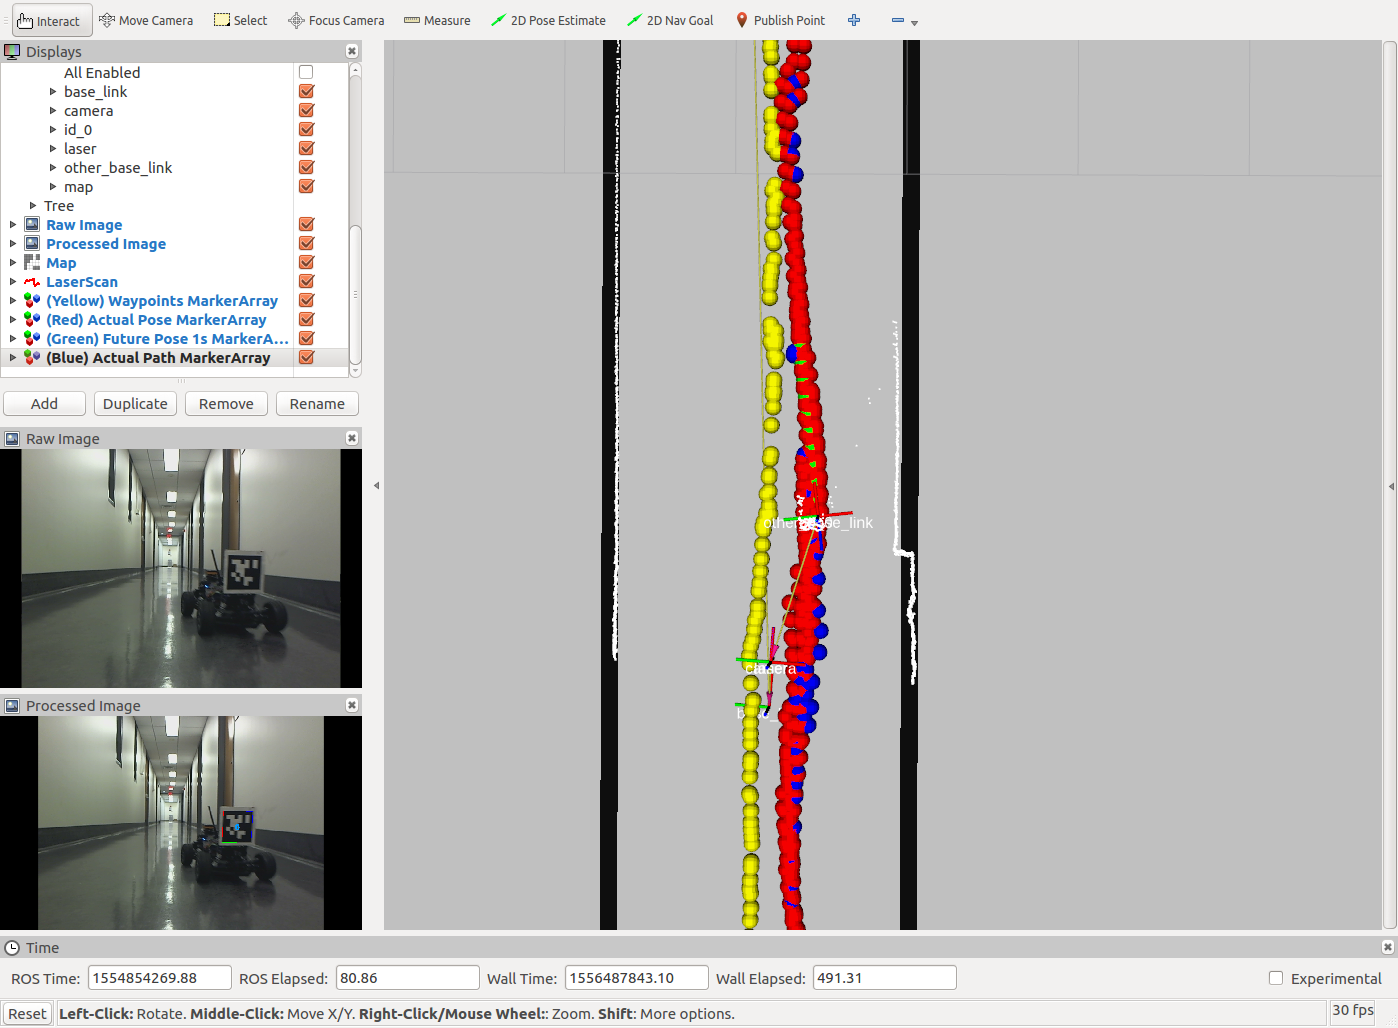
\includegraphics[width=\textwidth]{actual-versus-predicted-path-13.png}
		\caption{Tracking and predicting the pose of an opponent}
		\label{fig:overview}
	\end{figure}
	
	\section{Working with AprilTags}
	\subsection{Download the required packages }
	You can download the package containing the required repositories from this link. \href{https://drive.google.com/open?id=1yCs7dbwPPBzjbPul1k0SwnOg4jth4hTx}{Link}
	\subsection{Obtain camera parameters}
	The camera parameters and rviz parameters are present in the config/ folder of the repository.
	
	\subsection{Install apriltag\_ros}
	Download the required base repositories from this link \href{https://github.com/AprilRobotics/apriltag}{base April Tags}. There are instructions for setting up the base april tags repository. 
	First set up the AprilTag repositories, then You will just have to include the folders in the zip file in you src/ folder and compile your workspace. 
	
	\begin{lstlisting}[language=bash]
	$ catkin_make
	\end{lstlisting}
	
	
	\subsection{Set up vehicle tracker and prediction repository}
	Once you have AprilTags setup you have to work on the vehicle\_tracking\_prediction repository. Verify that there are no missing dependancies.If the dependencies are installed correctly there should be no compiler errors.\\
	Now you will be able to test the basic functionality of the AprilTags library. First, start playback of the recorded sensor data:
	\begin{lstlisting}[language=bash]
	$ rosbag play <bagfile>
	\end{lstlisting}
	Then launch the AprilTag detector:
	\begin{lstlisting}[language=bash]
	$ roslaunch vehicle_tracker_prediction_skeleton detect_apriltags.launch
	\end{lstlisting}
	
	\begin{figure}
		\centering
		% replace sample_figure.png with your image file in this folder
		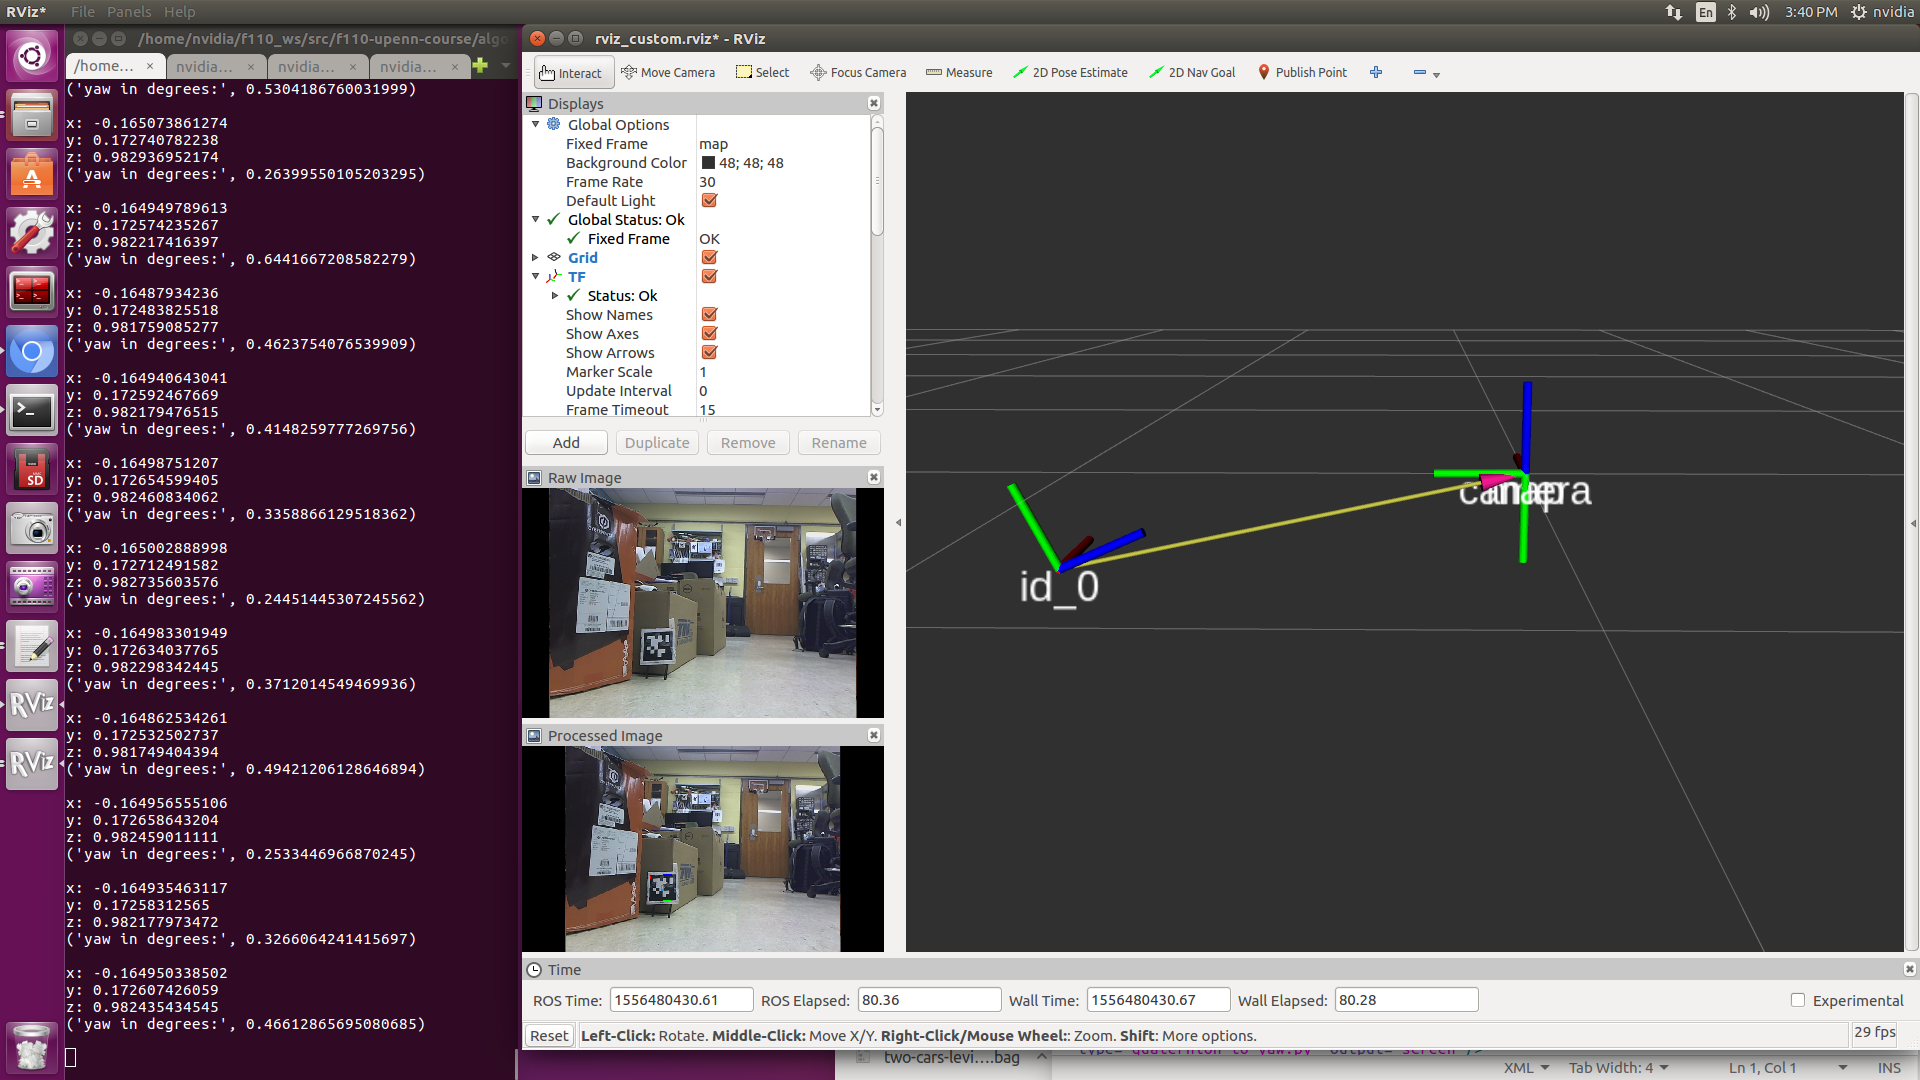
\includegraphics[width=0.5\textwidth]{detect-apriltag-launch.png}
		\caption{Detecting April Tags over Rviz}
	\end{figure}
	
	The next step is to modify the following files in the repository
	
	\begin{lstlisting}[language=bash]
	1. Vehicle_Track.cpp
	\end{lstlisting}
	The following tasks need to be performed by the pose predictor node: 
	\begin{itemize}
		\item It should subscribe to /tag\_detections topic with AprilTagsArray message type.
		\item It should implement the weighted prediction algorithm described in lecture. 
		\item You should tune the weighted prediction hyperparameters.
		\item It should publish the poses to a topic called /pose\_predictions which will have a markerarray message type. 
	\end{itemize}{}
	
	\subsection{Deliverables}
	You should submit the updated vehicle tracker package and clear instructions on how to run your code including any additional dependencies or libraries (e.g. Pure Pursuit implementation).
	
	\clearpage
	\section{Convert Nodes to Nodelets}
	Using nodelets is a standard practice when it comes to working with images in ROS. Transporting image messages over the standard TCP protocol for pub/sub in ROS creates significant delays. Instead of creating copies of images and passing the data around, nodelets creates shared memory between nodes and pass the pointer to the image in memory instead under a nodelet manager.
	The apriltag\_ros wrapper we provided does not run on nodelets, and is not fast enough to provide a robust detection framework. You'll need to convert the bare apriltag\_ros package to run on nodelets.
	\textbf{Warning:} Please do not copy any existing code that you can find on the internet to convert to nodelets. We will know if you copied from existing repositories online.\\

	
	\noindent\textit{References: }\\
	\href{http://wiki.ros.org/nodelet}{ROS wiki}\\
	\href{http://tayyabnaseer.blogspot.com/2013/04/porting-nodes-to-nodelets-in-ros.html}{Blog on porting nodes to nodelets}\\
	\href{https://github.com/cryborg21/sample_nodelet/tree/master/src}{Example nodelet}\\
	\href{https://www.clearpathrobotics.com/assets/guides/ros/Nodelet\%20Everything.html}{Clearpath robotics tutorial}\\
	
	Here are a few steps and tips that you can take to get started.
	\begin{itemize}
		
		\item Everything you need to care about is in the ROS package inside the folder apriltags2\_ros
		
		\item Since we are only using the continuous\_detector node you can only convert this node into a nodelet. \item First, edit the continous\_detector.h file. You will have to make a shared pointer object for the TagDetector Object and also a shared pointed object image\_transoirt object. 
		\item  You will have to add the nodelet spec will ifications in the main function in the apriltags2\_ros\_continous\_node.cpp file. 
		\item In continuous\_node.cpp you will have explort the pluginlib class list macros and specify the class to be exported. You will have to make the oninit() function and initialize the nodehandles, tag detector objects, image transport objects, etc. inside it. You can now leave the constructor empty. Ypu might have to make some changes in the image callback function too. 
		\item in the cmake list you will have to take care of the dependencies such as pluginlib and nodelet. Make sure your executable and libraries are defined correctly for the continuous node detector
		\item You will create a new .xml file called the nodelet\_plugins.xml file and specify the library path and the class path. 
		\item You will change the package.xml file to specify the dependencies of nodelets and pluginlib and also export the nodelet\_plugins.xml file. This will be loaded during runtime. 

	\end{itemize}

	\section{Test Framework} 
	We have provided a launch file \texttt{bag\_prediction.launch} to test your system using a bag file. You may have to change some parameters in the launch file. 
	% \begin{lstlisting}[language=bash]
	% roslaunch Vehicle_tracker_prediction_skeleton bag_prediction.launch
	% \end{lstlisting}
	% \\
	The launch file will launch RViz in order to display the markers showing the poses which are estimated by the algorithm. Record a video of your predictions as displayed in RViz. In addition compare the frequency of messages published on the detected poses topic with and without the use of nodelets. \\
	In the launch file you will have to add the launch commands for the executable you create. The scripts/ folder also contains utilities that you can use to save and/or publish markers of the waypoints, predicted poses and actual poses. Feel free to use them. 
	
		\begin{figure}[h]
		\centering
		% replace sample_figure.png with your image file in this folder
		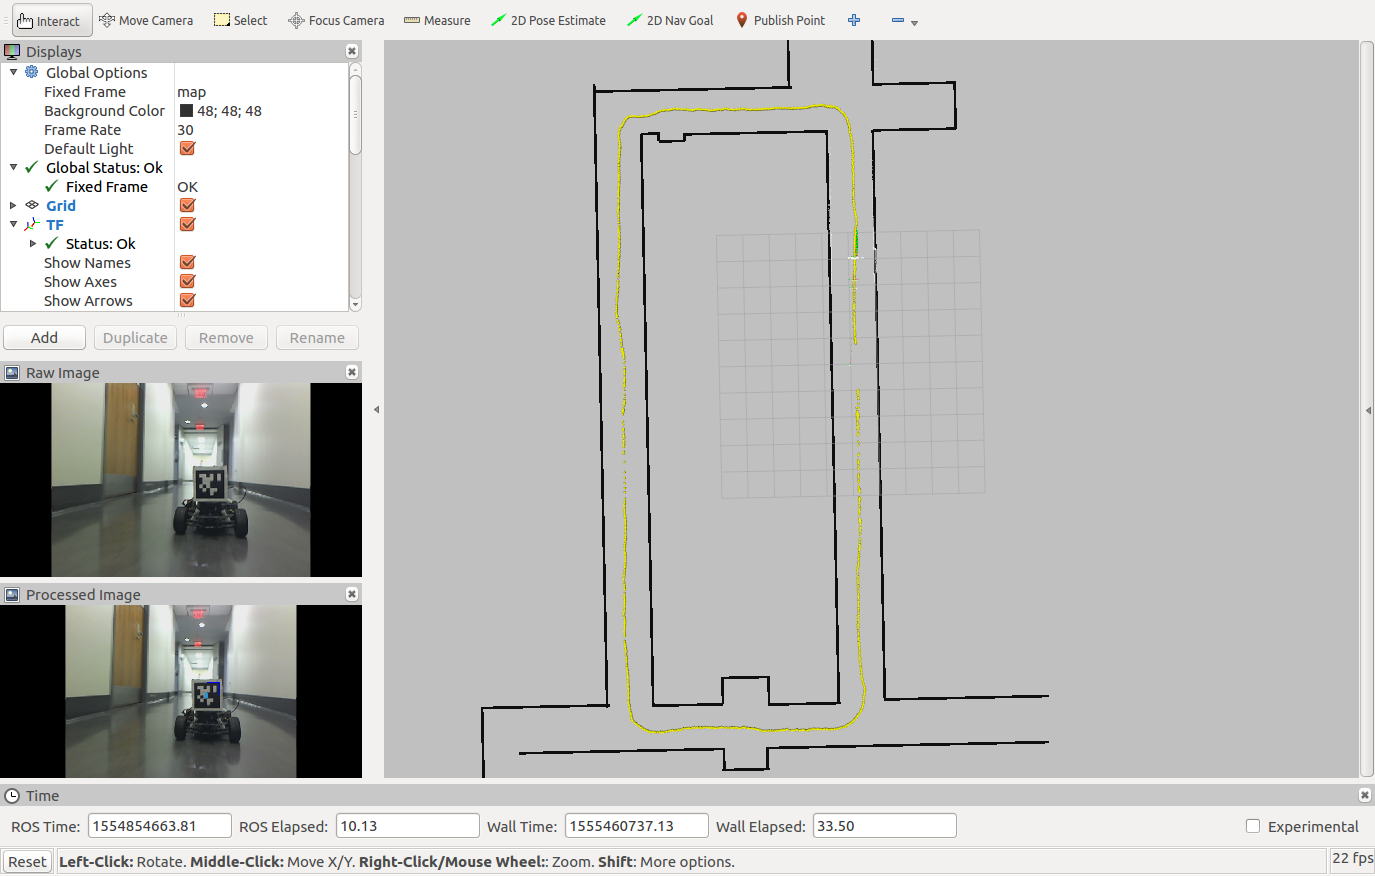
\includegraphics[width=0.5\textwidth]{waypoints.png}
		\caption{Predicting Poses over Rviz}
	\end{figure}

	\section{Extra Credit}
	You may already be doing some of these things for your project, this is some encouragement to get started early. The mechanical design and TX2 kernel support tasks have slightly flexible deadlines, see your TAs. The other tasks must be submitted with your lab to receive the bonus points. Extra credit will be awarded on an individual basis. If multiple team members participate you must use git to track contributions and supply the teaching staff with relevant commit history and a summary of who did what. The teaching staff's decisions about partially completed tasks and sufficiency of contributions by an individual working in a team are final. 
	
	\subsection{Mechanical Design} \textit{\textbf{(10 pts added to lowest lab score)}}
	
	\noindent Create a 3D printed mount for the realsense or logitech cameras
	\newline
	
	\noindent\textit{\textbf{(10 pts added to lowest lab score)}}
	
	\noindent Create a mount for placing an AprilTag on the back of the car (3D printed and laser cut)
	\newline
	
	\noindent\textit{\textbf{(10 pts added to lowest lab score)}}
	
	\noindent Fabricate the designs for the rest of the class once submitted (you need certification from MEAM to use these tools). 
	
	\subsection{Improved Prediction} \textit{\textbf{(5 pts added to lowest lab score)}}
	
	\noindent Use RRT, RRT$^{*}$, or follow-the-gap instead of pure-pursuit within the prediction algorithm. Can you weight the predictions from multiple algorithms? How would you decide the weighting etc. 
	\newline
	
	\noindent\textit{\textbf{(10 pts added to lowest lab score)}}
	
	\noindent Use MPCC within the prediction algorithm. 
	
	\subsection{Update the TX2 Kernel to support RealSense Camera} \textit{\textbf{(5 pts added to lowest lab score)}}
	
	\noindent Provide a script and verify with the TAs so we can distribute this to the rest of the class. Be careful, hacking without understanding can brick your TX2. 
	
	\subsection{YOLO pipeline}\textit{\textbf{(10 pts added to lowest lab score)}}
	
	\noindent Replace the AprilTags pipeline with YOLO keep output of detected poses the same etc. 


	\section{Deliverables and Submission}
	% Make sure to place "labx" below with the correct lab number
	Submit the following as \texttt{groupnumber\_lab8.zip} (replace \texttt{number} with your groupnumber):
	

	\begin{enumerate}
		\item Your nodelet implementation of the vehicle tracker package and clear instructions on how to run your code including any additional dependencies or libraries (e.g. Pure Pursuit implementation).
		\item A youtube video of your detection and prediction pipeline. Add this link to a text file named \texttt{groupnumber\_lab8\_video.txt}
		\item A plot showing the mean and variance of the detected poses publishing frequency.
	\end{enumerate}

	\section{Grading}
	
	
	\subsection{Rubric}
	\begin{table}[h]
		\begin{tabular}{ll}
			\textbf{Topics} & \textbf{Points} \\
			Compilation & 10 \\
			Tracking implementation	& 30 \\
			tracking performance on turns &	10 \\
			Nodelets Implementation &	25 \\
			Nodelets: improvement in performance &	10 \\
			Video Provided &	10 \\
			Clear Instructions and Readme &	5 \\
			Extra credit 	&  0 \\
			\textbf{Total} & 100 \\
		\end{tabular}
	\end{table}
	

	
			
\end{document} 
